\section{Métodos en diferencias finitas}
En esta sección vamos a ver métodos en diferencias finitas para distintos tipos de ecuaciones. Estos métodos se utilizan para calcular las soluciones aproximadas a las ecuaciones diferenciales aproximando derivadas.

\subsection{Ecuaciones parabólicas en una dimensión espacial.}
Este tipo de ecuaciones tiene la forma:
$$e(x,t)u_t = \underbrace{\frac{\partial}{\partial x} \left(a(x,t)\frac{\partial u}{\partial x}\right)}_{t_d} + \underbrace{b(x,t)\frac{\partial u}{\partial x}}_{t_c}+\underbrace{c(x,t)u}_{t_n} + \underbrace{d(x,t)}_{t_f}$$
 
para $x\in I, t>0$.

Donde:
\begin{itemize}
	\item $a,b,c,d,e$: funciones proporcionadas.
	\item $x$: variable espacial.
	\item $t$: variable temporal.
	\item $t_d$: término de difusión.
	\item $t_c$: término conectivo.
	\item $t_n$: término de reacción.
	\item $t_f$: término fuente.			
\end{itemize}

Vamos a tratar con los siguientes tipos de condiciones de contorno:
\begin{itemize}
	\item \textbf{Condición de Dirichlet}	
	\begin{equation*}
		\begin{array}{l l}
			u(a,t) = f_1(t)\\
			u(b,t) = f_2(t)\\
		\end{array}
	\end{equation*}
	Se denominan condiciones homogéneas si $f_1=f_2=0$.
	\item \textbf{Condición de Neumann}	
	\begin{equation*}
		\begin{array}{l l}
			u_x(a,t) = g_1(t)\\
			u_x(b,t) = g_2(t)\\
		\end{array}
	\end{equation*}
	Se denominan condiciones homogéneas si $g_1=g_2=0$.
\end{itemize}

\subsubsection{La ecuación del calor}
La ecuación del calor es un caso particular de ecuación parabólica en una dimensión espacial en la que $u(x,t)$ representa el valor de la temperatura en tiempo $t$ en el punto $x$.

Supongamos que tenemos una barra unidimensional de cualquier material cuyos extremos se localizan en los puntos $0$ y $1$.

El problema se define como sigue:
\begin{equation*}
	\left\{
	\begin{array}{l l l}
		u_t = u_{xx} & x\in(0,1), t>0\\
		u(0,t) = u(1,t) = 0 & \text{Temperatura en los extremos.}\\
		u(x,0) = u_0(x) & \text{Temperatura en el tiempo inicial.}\\
	\end{array}
	\right.
\end{equation*}

Vamos a utilizar el método de separación de variables para encontrar la solución. Para ello supongamos que la solución se puede representar como el producto de dos funciones $f(x)$ y $g(t)$, es decir $u(x,t) = f(x)g(t)$.

Como $u_t = u_{xx}$, derivando $u(x,t)$ respecto a $t$ una vez, respecto a $x$ dos veces e igualando términos, obtenemos:
$$f(x) \dot{g}(t) = \ddot{f}(x) g(t)$$
de donde si despejamos obtenemos una igualdad en la que el término izquierdo depende de $t$ y el derecho de $x$. Si se deriva el término izquierdo respecto a $x$ se obtiene cero igualmente que si derivamos el derecho respecto a $t$. Con esto obtenemos que los términos no dependen ni de $x$ ni de $t$, luego son iguales a una constante que por comodidad para cálculos posteriores denotaremos como $-K^2$:
$$\frac{\dot{g}(t)}{g(t)} = \frac{\ddot{f}(x)}{f(x)} = cte = -K^2$$
Tenemos entonces dos ecuaciones diferenciales ordinarias:
\begin{equation*}
	\left\{
	\begin{array}{l}
		\ddot{f}(x) = -K^2 f(x)\\
		\dot{g}(t) = -K^2 g(t)\\
	\end{array}
	\right.
\end{equation*}
Al resolver las ecuaciones se obtiene
\begin{equation*}
	\begin{array}{l}
		f(t) = Acos(Kx) + Bsin(Kx)\\
		g(t) = e^{-K^2 t}
	\end{array}
\end{equation*}
Las condiciones de contorno establecían que $u(0,t) = u(1,t) = 0$. 
Dado que hemos supuesto que $u(x,t) = f(x)g(t)$ se esta imponiendo que $f(0) = f(1) = 0$, lo que implica que
\begin{equation*}
	\left\{
	\begin{array}{l}
		f(0) = Acos(0) + Bsin(0) = 0\\
		f(1) = Acos(K) + Bsin(K) = 0\\
	\end{array}
	\right.
\end{equation*}
Esto sólo puede ocurrir si
\begin{equation*}
	\left\{
	\begin{array}{l l}
		A = 0 & \\
		K = m\pi & m\in\mathbb{Z}\\
	\end{array}
	\right.
\end{equation*}
Como la condición se satisface $\forall m \in \mathbb{Z}$ tenemos infinitas funciones $f_m, g_m$ que cumplen la condición. Luego para cada $m$, se tiene que $u_m(x,t) = f_m(x)g_m(t)$ es solución del problema de contorno.
Por tanto también lo es
$$u(x,t) = \sum_{m=1}^\infty B_m e^{-(m\pi)^2 t} sin(m\pi x)$$
donde $B_m$ es una constante que depende de $m$.

Sin embargo, hasta ahora sólo se han tenido en cuenta las condiciones de contorno y no la condición inicial. Hay que imponer dicha condición para obtener una solución al problema. Dicha condición establece que $u(x,0) = u_0(x)$ siendo $u_0$ una función proporcionada.
Tenemos que:
$$u(x,0) = u_0(x) = \sum_{m=1}^\infty B_m sin(m\pi x)$$
Lo que nos dice que los términos $B_m$ son los coeficientes del desarrollo en senos de la serie de Fourier de $u_0$.
Es decir, que:
$$\int_0^1 u_0(x) sin(m\pi x) = B_m \int_0^1 sin^2(m\pi x) = \frac{B_m}{2}$$ para cada $m\in\mathbb{Z}$. Obteniendo así $$B_m = 2\int_0^1 u_0(x) sin(m\pi x)$$
Finalmente, la solución general al problema completo es:
$$u(x,t) = \sum_{m=1}^\infty B_m e^{-(m\pi)^2 t} sin(m\pi x)$$ donde $B_m$ tiene la expresión definida anteriormente.

En caso de que tuviesemos un dato inicial $u_0$ y quisiésemos hallar la solución del problema de la ecuación del calor tendríamos que

\begin{itemize}
	\item Hallar el valor aproximado de la serie, para lo cual se evalua cada término para cada $m$ y se trunca la serie cuando se considere que se ha obtenido un resultado muy pequeño.
	\item Para lo anterior es necesario hallar el valor de $B_m$ para cada iteración, bien de forma exacta si es posible o mediante métodos numéricos. Una opción sería utilizar cuadratura numérica:
	$$\int_a^b f(x) \approx \sum_{j=0}^k w_j f(x_j)$$
\end{itemize}

\paragraph{Método explícito}
En este apartado se va a describir un método explícito para la ecuación del calor: el método en diferencias finitas.

En primer lugar se construyen dos particiones para cada variable, una para el intervalo $(0,1)$ y otra para el intervalo $(0,t_f)$ donde $t_f$ representa el tiempo final, de forma que $x\in(0,1)$ y $t\in(0,t_f)$.

Cada partición se define a través de los valores del paso, que son
\begin{equation*}
	\begin{array}{lll}
		\Delta x = \frac{1}{J}& \textbf{y} & \Delta t = \frac{t_f}{N}
	\end{array}
\end{equation*}
donde $J,N\in\mathbb{N}$, es decir, que se obtienen $N+1$ puntos en $(0,1)$ y $J+1$ puntos en $(0,t_f)$:
\begin{align*}
0=x_0<x_1<\hdots<x_J = 1\\
0=t_0<t_1<\hdots<t_N = t_f
\end{align*}

\begin{mdframed}
	\textbf{Notación:}
	\begin{itemize}
		\vspace{-3mm}
	\item $U_j^n$ representa el valor de la función $u$ evaluada en $(x_j,t_n)$ obtenida por el método.
	\item $u_j^n$ representa el valor \textbf{real} de la función $u$ evaluada en $(x_j,t_n)$.
	\end{itemize}
\end{mdframed}

Las condiciones de contorno del problema imponían que 
$$u(0,t) = u(1,t) = 0$$
luego
\begin{equation*}
	\left\{
	\begin{array}{l}
	u_0^n = U_0^n = 0, n\ge 0\\
	u_J^n = U_J^n = 0, n\ge 0
	\end{array}
	\right.
\end{equation*}
El método es el siguiente
\begin{equation*}
	\frac{U_j^{n+1}-U_j^n}{\Delta t} =  \frac{U_{j+1}^n-2U_j^n+U_{j-1}^n}{(\Delta x)^2}
\end{equation*}
para $n\ge  0, j=1,\hdots ,J-1$.

\noindent Si definimos
$\nu = \frac{\Delta t}{(\Delta x )^2}$ y despejamos lo anterior, obtenemos el método explícito.
\begin{mdframed}
	\textbf{Método explícito}
	$$U_j^{n+1} = U_j^n+\nu\left(U_{j+1}^n - 2 U_j^n + U_{j-1}^n\right)$$
\end{mdframed}
Veamos de donde sale el método. Supongamos que $u(x)$ es una solución del problema. Aplicando el método obtenemos lo siguiente: 

\begin{equation*}
	\begin{array}{r l l}
	\frac{u(x_j, t_{n+1})-u(x_j,t_n)}{\Delta t} &\approx& u_t(x_j, t_n) + \hdots\\
	\frac{u(x_{j+1}) - 2u(x_j, t_n) + u(x_{j-1}, t_n)}{(\Delta x)^2} &\approx& u_{xx}(x_j, t_n) + \hdots
	\end{array}
\end{equation*}
Vamos a ver con el desarrollo de la serie Taylor qué orden tiene esta aproximación.

\subparagraph*{Derivada temporal} 
\mbox{}

Tenemos que:
$$u(x_j, t_{n+1}) = u(x_j, t_n) + u_t(x_j, t_n)\Delta t +\frac{u_{tt} (x_j,t_n)}{2}\Delta t ^2 + O\left((\Delta t)^3\right)$$

luego:
$$\frac{u(x_j,t_{n+1}) - u(x_j, t_n)}{\Delta t} = u_t(x_j,t_n) + \underbrace{\frac{\Delta t}{2} u_{tt}(x_j,t_n) + O\left((\Delta t)^2\right)}_{\text{error}}$$

\subparagraph*{Derivada espacial} 
\mbox{}

Tenemos que:
\begin{equation*}
\begin{array}{lll}
u(x_{j+1}, t_n) &=& u(x_j,t_n) + u_x(x_j,t_n)\Delta x + u_{xx}(x_j,t_n)\frac{\Delta x^2}{2}\\ &&+\  u_{xxx}(x_j,t_n)\frac{\Delta x^3}{3!}  + \hdots\\
u(x_{j-1},t_n) &=& u(x_j, t_n) - u_x(x_j,t_n)\Delta x + u_{xx}(x_j,t_n)\frac{(\Delta x)^2}{2}\\ &&-\ u_{xxx}(x_j, t_n)\frac{(\Delta x)^3}{3!} + u_{xxxx}(x_j,t_n)\frac{(\Delta x)^4}{4!} + \hdots
\end{array}
\end{equation*}

luego:
$$\frac{u(x_{j+1}, t_n) - 2u(x_j,t_n) + u(x_{j-1},t_n)}{(\Delta x)^2} = u_{xx}(x_j,t_n) +  u_{xxxx}(x_j, t_n)\frac{\Delta x^2}{12} + O\left((\Delta x)^4\right)$$

Como conclusión tenemos que el método explícito utiliza una diferencia finita de primer orden para aproximar la derivada temporal y una diferencia finita de segundo orden para aproximar la derivada espacial.

\begin{defn}[Error de truncacion]
Se llama error de truncación del método numérico al residuo que se obtiene cuando se aplica el método a la solución exacta.
\end{defn}
\begin{equation*}
\begin{array}{l l l}
T(x_j,t_n) &=& \frac{u(x_j,t_{n+1})-u(x_j,t_n)}{\Delta t} - \frac{u(x_{j+1},t_n)-2u(x_j,t_n)+u(x_{j-1},t_n)}{\Delta x^2}\\ 
& = & u_t(x_j,t_n) + u_{tt}(x_j,t_n)\frac{\Delta t}{2} + O \left((\Delta t)^2\right) \\
&& -\ u_{xx}(x_j,t_n) + u_{xxxx}(x_j,t_n)\frac{\Delta x^2}{12} + O\left((\Delta x)^4\right)\\ 
& = & u_{tt}(x_j,t_n)\frac{\Delta t}{2} -  u_{xxxx}(x_j,t_n)\frac{\Delta x^2}{12} + O\left((\Delta t)^2\right) + O\left((\Delta x)^4\right)
\end{array}
\end{equation*}
Otra forma de escribirlo es
$$T_j^n = \Delta t \left(\frac{u_{tt}(x_j,t_n)}{2}- \frac{1}{12\nu} u_{xxxx}(x_j,t_n)\right) + O\left((\Delta t)^2\right) + O\left((\Delta x)^4\right)$$

Si tomamos $\xi_n \in (t_n,t_{n+1})$ y $\eta_j \in (x_{j-1}, x_{j+1}):$

$$T_j^n = \Delta t \left(\frac{u_{tt}(x_j,\xi_n)}{2}- \frac{1}{12\nu} u_{xxxx}(\eta_j,t_n)\right)$$

\subparagraph*{Cota para el error de truncación}

Si tomamos $M_{tt}$ y $M_{xxxx}$ como cota para $u_{tt}$ y $u_{xxxx}$, tenemos el error de truncación acotado por

$$|T_j^n| \le \Delta t \left(\frac{M_{tt}}{2} + \frac{M_{xxxx}}{12{\nu}}\right)$$

Si $u_{t} = u_{xx}$ entonces $u_{tt} = (u_{t})_{xx} = u_{xxxx}$

\subparagraph*{Caso particular}
\mbox{}

Si $\nu = 1/6$
$$T_j^n = O\left((\Delta t)^2\right) + O\left((\Delta x)^4\right) = O\left((\Delta t)^2\right)$$ 

porque 
$\Delta t = \nu (\Delta x )^2$

El método explícito es consistente porque el error de truncación tiende a cero cuando $\Delta t \to 0$.
Además es incondicionalmente consistente, lo que quiere decir que $T_j^n$ tiende hacia cero independientemente de los valores de $\Delta t$ y $\Delta x$ (más concretamente de su relación).

\begin{prop}
	Estabilidad  $+$ Consistencia $\iff$ Convergencia.
\end{prop} 

A partir de esta proposición y dado que el método es incondicionalmente consistente, basta que sea estable para que sea convergente.

\begin{prop}
El método es estable $\iff$ $\nu = \frac{\Delta t}{\left(\Delta x\right)^2} \le \frac{1}{2}$
\end{prop}

\begin{proof}
	
Vamos a ver, utilizando el principio del máximo, que si $\nu < 1/2$, el método es estable. Tenemos que:
\begin{equation*}
\begin{array}{lll}
U_j^{n+1} &=& U_j^n + \nu (U_{j+1}^n-2U_j^n+U_{j-1}^n)\\
u_j^{n+1} &=& u_j^n + \nu (u_{j+1}^n-2u_j^n+u_{j-1}^n) + T_j^n \Delta t
\end{array}
\end{equation*}

Denotamos con $e_j^n$ al residuo del método de forma que
$$e_j^n = U_j^n - u_j^n$$

Calculamos el error de paso:
$$e_j^{n+1} = e_j^n + \nu (e_{j+1}^n-2e_j^n+e_{j-1}^n) - T_j^n \Delta t$$

Que reescrito de otro modo y suponiendo que $\nu \le \frac{1}{2}$ queda:
$$e_j^{n+1} = \nu e_{j+1}^n + \underbrace{(1-2\nu)}_{\ge 0} e_j^n + \nu e_{j-1}^n - T_j^n \Delta t$$

Ahora definimos
$$E^n = \max_{0\le j \le J} |e_j^n|$$

para acotar el error
\begin{equation*}
	\begin{array}{lll}
	|e_j^{n+1}| &\le& \nu|e_{j+1}^n| + (1-2\nu) |e_j^n| + \nu |e_{j-1}^n| +  \bar{T}\Delta t\\
	&\le& \nu E^n +(1-2\nu)E^n + \nu E^n + \bar{T}\Delta t\\
	&=& E^n + \bar{T} \Delta t
	\end{array}
\end{equation*}

Donde $$\bar{T} = \Delta t \left( \frac{M_{tt}}{2} + \frac{M_{xxxx}}{12\nu}  \right)$$

es decir, $\bar{T}$ es la cota para el error de truncación. 

\subparagraph*{Conclusión}
\begin{equation*}
	\left\{
	\begin{array}{llll}
	E^0 &=& 0&\\
	E^n &=& n\Delta t \bar{T}\ & \le\ t_f \bar{T}\\	
	E^n &\to& 0 &\text{cuando }\Delta t \to 0
	\end{array}
	\right.
\end{equation*}
\end{proof}

\subparagraph*{Programación del método}
Sabemos que inicialmente tenemos los siguientes datos
\begin{equation*}
	\left\{
	\begin{array}{l r}
		u(0,t) = 0\\
		u(1,t) = 0\\
		u(x,0) = u_0(x)
	\end{array}
	\right.
\end{equation*}

Es decir, que disponemos de los datos iniciales (en tiempo $t=0$) y de contorno (cuando $x=0$ y $x=1$). Partiendo de estos podemos calcular el resto de datos como ya hemos visto:

$$U_j^{n+1} = U_j^n+\nu\left(U_{j+1}^n - 2 U_j^n + U_{j-1}^n\right)$$

\begin{figure}[h]
	\centering
	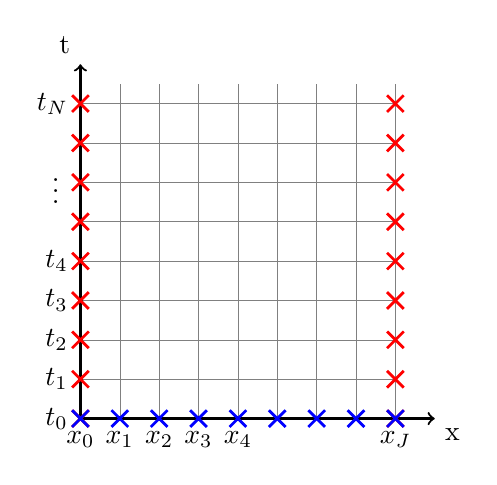
\begin{tikzpicture}[domain=0:4]
	%Grid
	\draw[step=5mm,very thin,color=gray] (0,0) grid (4,4.25);
	%Axis
	\draw[thick,->] (0,0) -- (4.5,0) node[below right] {x};
	\draw[thick,->] (0,0) -- (0,4.5) node[above left] {t};
	\foreach \x in {0,1,2,3,4}
	\draw (5*\x mm,1pt) -- (5*\x mm,-1pt) node[below] {$x_\x$};
	\node[below] at (3,-4pt){$\hdots$};
	\node[below] at (4,-1pt){$x_J$};
	\foreach \y in {0,1,2,3,4}
	\draw (1pt,5*\y mm) -- (-1pt,5*\y mm) node[left] {$t_\y$};
	\node[left] at (-4pt,3){$\vdots$};
	\node[left] at (-1pt,4){$t_N$};
	%Data
	\foreach \x in {0,...,8}{
		\draw[rotate around={45:(0,5*\x mm)},red, line width=1pt] (0.15,5*\x mm) -- (-0.15,5*\x mm);
		\draw[rotate around={135:(0,5*\x mm)},red, line width=1pt] (0.15,5*\x mm) -- (-0.15,5*\x mm);
	}
	\foreach \x in {0,...,8}{
		\draw[rotate around={45:(4,5*\x mm)},red, line width=1pt] (4.15,5*\x mm) -- (3.85,5*\x mm);
		\draw[rotate around={135:(4,5*\x mm)},red, line width=1pt] (4.15,5*\x mm) -- (3.85,5*\x mm);
	}
	\foreach \y in {0,...,8}{
		\draw[rotate around={45:(5*\y mm,0)},blue, line width=1pt] (5*\y mm,0.15) -- (5*\y mm,-0.15);
		\draw[rotate around={135:(5*\y mm,0)},blue, line width=1pt] (5*\y mm,0.15) -- (5*\y mm,-0.15);
	}
	\end{tikzpicture}
	\caption{Datos iniciales y de contorno}
	\label{fig:calor_1}
\end{figure}

Gráficamente, los datos que tenemos se pueden ver en la figura \ref{fig:calor_1}. En color rojo se muestran los datos de contorno, que en este caso son todos $0$ puesto que tenemos $u(0,t) = u(1,t) = 0$. En color azul se muestran los datos iniciales, que corresponden con los valores de la función proporcionada $u_0(x)$. En la figura también se puede ver cómo se ha realizado un mallado del espacio para aplicar el método.

A partir de estos datos se construye el algoritmo vectorial de la siguiente forma:
\begin{equation*}
	\begin{array}{l l l}
		\begin{bmatrix}
			U_1^{n+1}\\
			U_2^{n+1}\\
			\vdots\\
			U_{j-1}^{n+1}\\
		\end{bmatrix}
		=
		\begin{bmatrix}
			1-2\nu & \nu       &        & \\
			\nu    & \ddots    & \ddots & \\
			          & \ddots & \ddots & \nu\\
			          &        & \nu    & 1-2\nu\\
		\end{bmatrix}
		\begin{bmatrix}
			U_1^{n}\\
			U_2^{n}\\
			\vdots\\
			U_{j-1}^{n}\\
		\end{bmatrix}
	\end{array}
\end{equation*}

Gráficamente, lo que estamos realizando es obtener una aproximación (utilizando la aproximación de las derivadas) del siguiente punto de la partición en la derivada temporal a partir del punto anterior, el actual y el siguiente en la derivada espacial (ver figura \ref{fig:calor_2}). De esta forma, sólo usando los datos iniciales y de contorno obtenemos un valor para cada uno de los puntos del mallado.

\begin{figure}[h]
	\centering
	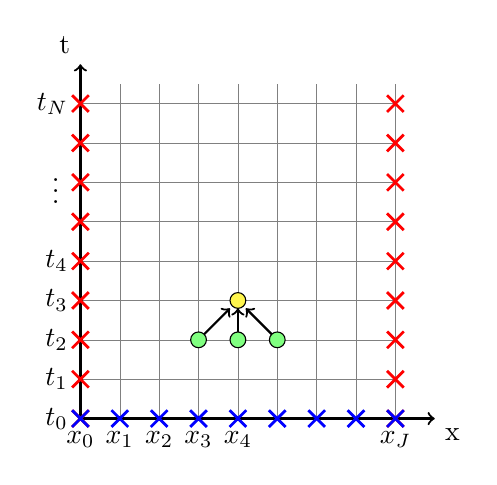
\begin{tikzpicture}[domain=0:4]
	%Grid
	\draw[step=5mm,very thin,color=gray] (0,0) grid (4,4.25);
	%Axis
	\draw[thick,->] (0,0) -- (4.5,0) node[below right] {x};
	\draw[thick,->] (0,0) -- (0,4.5) node[above left] {t};
	\foreach \x in {0,1,2,3,4}
	\draw (5*\x mm,1pt) -- (5*\x mm,-1pt) node[below] {$x_\x$};
	\node[below] at (3,-4pt){$\hdots$};
	\node[below] at (4,-1pt){$x_J$};
	\foreach \y in {0,1,2,3,4}
	\draw (1pt,5*\y mm) -- (-1pt,5*\y mm) node[left] {$t_\y$};
	\node[left] at (-4pt,3){$\vdots$};
	\node[left] at (-1pt,4){$t_N$};
	%Data
	\foreach \x in {0,...,8}{
		\draw[rotate around={45:(0,5*\x mm)},red, line width=1pt] (0.15,5*\x mm) -- (-0.15,5*\x mm);
		\draw[rotate around={135:(0,5*\x mm)},red, line width=1pt] (0.15,5*\x mm) -- (-0.15,5*\x mm);
	}
	\foreach \x in {0,...,8}{
		\draw[rotate around={45:(4,5*\x mm)},red, line width=1pt] (4.15,5*\x mm) -- (3.85,5*\x mm);
		\draw[rotate around={135:(4,5*\x mm)},red, line width=1pt] (4.15,5*\x mm) -- (3.85,5*\x mm);
	}
	\foreach \y in {0,...,8}{
		\draw[rotate around={45:(5*\y mm,0)},blue, line width=1pt] (5*\y mm,0.15) -- (5*\y mm,-0.15);
		\draw[rotate around={135:(5*\y mm,0)},blue, line width=1pt] (5*\y mm,0.15) -- (5*\y mm,-0.15);
	}
		\draw[thick,->] (1.5,1) -- (1.9,1.4);
		\draw[thick,->] (2,1) -- (2,1.4);
		\draw[thick,->] (2.5,1) -- (2.1,1.4);
	\draw[fill=green!50!white, draw=black] (1.5,1) circle (1mm);
	\draw[fill=green!50!white, draw=black] (2,1) circle (1mm);
	\draw[fill=green!50!white, draw=black] (2.5,1) circle (1mm);
	\draw[fill=yellow!70!white, draw=black] (2,1.5) circle (1mm);
	\end{tikzpicture}
	\caption{Método en diferencias finitas: $U_j^{n+1} = U_j^n+\nu\left(U_{j+1}^n - 2 U_j^n + U_{j-1}^n\right)$}
	\label{fig:calor_2}
\end{figure}

\subparagraph*{Análisis de Fourier del método}
Hemos visto que
$$u(x, t) = \sum_{m=1}^\infty B_m e^{-(m\pi)^2 t} sin(m\pi x)$$
Lo que es equivalente a escribir
$$u(x,t) = \sum_{m=-\infty}^\infty B_m e^{-(m\pi)^2 t}e^{i(m\pi)x}$$
Para la solución teórica, los modos de Fourier
\begin{equation*}
	\begin{array}{l c r}
	e^{-k^2t} & \text{y} &e^{ikx}
	\end{array}
\end{equation*}
con $k=m\pi$ y $m=-\infty,\hdots,\infty$,
son soluciones.
Tomando el factor de amplificación 
$$\lambda(k) \simeq e^{-k^2\Delta t}$$ necesitamos que 
\begin{equation*}
	\begin{array}{l l l}
		U_j^n = \lambda^n e^{ik(j\Delta x)} &\simeq& e^{-k^2t_n}\ e^{ikx_j}\\
				&=& e^{-k^2n\Delta t}\ e^{ik_k\Delta x}\\
				&=& \left[e^{-k^2\Delta t}\right]^n\ e^{ik_j\Delta x}
	\end{array}
\end{equation*}
Sustituyendo en el método tenemos que
$$\lambda^{n+1}e^{ik_j\Delta x} =
\lambda^ne^{ik_j\Delta x} + \nu\left[\lambda^n e^{ik(j+1)\Delta x}-2\lambda^n e^{ik_j\Delta x}+\lambda^n e^{ik(j-1)\Delta x}\right]$$

Dividiendo por $\lambda^n e^{ik_j\Delta x}$

% %$$\lambda = 1+\nu\left[e^{ik\Delta x -2 + }\right]

% %

Tomando $U_j^n = \lambda(k)^n e^{ik_j\Delta x}$ se verifica el método.

Como aproximación al método, tomamos
$$U_j^n = \sum_{-\infty}^\infty B_m \lambda(k)^n e^{ik_j\Delta x}$$

Vamos a analizar el comportamiento cualitativo de $\lambda(k)$.

Si $|\lambda(k)| > 1 \implies |\lambda(k)|^n \to \infty$. Es decir, tenemos inestabilidad.

Tenemos estabilidad $\iff |\lambda(k)| \le 1$. Esto es equivalente a decir que podemos acotar dos aproximaciones numéricas del método en términos de los datos iniciales.

Tomamos

$$U_j^1 = \sum A_m^1 \lambda(k)^n e^{ik_j\Delta x}$$
$$U_j^2 = \sum A_m^2 \lambda(k)^n e^{ik_j\Delta x}$$

$$u_0^1 = \sum A_m^1 e^{ikx}$$
$$u_0^2 = \sum A_m^2 e^{ikx}$$

$$U_j^1 - U_j^2 = \sum_{-\infty}^\infty (A_m^1-A_m^2) \lambda(k)^n e^{ik_j\Delta x}$$

$$|U_j^1-U_j^2| \le \sum_{m=1}^\infty (A_m^1-A_m^2) e^{ik_j\Delta x} = u_0^1-u_0^2$$

Vamos a ver el comportamiento cuantitativo de $\lambda(k)$.

Comparación de $e^{-k^2\Delta t}$ y $\lambda(k)$.

$e^{-k^2\Delta t} = 1-k^2\Delta t + \frac{1}{2}k^4\Delta t ^2 + O(\Delta t ^3)$

$\lambda(k) = 1-4\nu sin^2(\frac{k}{2}\Delta x) = 1-4\nu\left[\frac{k^2}{4}\Delta x^2 - \frac{1}{3}\frac{k^4}{16}\Delta x^4 + \hdots \right] = 1-k^2\Delta t + \frac{k^4}{12}\Delta t \Delta x^2$

$\lambda(k) - e^{-k^2\Delta t} = \frac{k^4}{12}\Delta t \Delta x^2 - \frac{k^4\Delta t}{2} + O(\Delta t ^3)$

En general 

$\lambda(k) - e^{-k^2\Delta t} = O(\Delta t^2)$
Es decir, que el método tiene orden 1 de consistencia.

Se puede ver mejor si lo reescribimos de la forma
$\lambda(k) - e^{-k^2\Delta t} = \left[\frac{k^4}{12\nu}-\frac{k^4}{2}\right]\Delta t^2 + O(\Delta t^3)$

Vemos de nuevo que si $\nu = \frac{1}{6}$ se tiene orden 2 de consistencia.

%Aparte
$sin(x) = x-\frac{x^3}{3!}+\hdots$
$sin^2(x) = sin^2(x) = sin(x) sin(x) = (x-\frac{x^3}{3!})(x-\frac{x^3}{3!}) = x^2-2\frac{x^4}{3!} +\hdots = x^2 - \frac{x^3}{3!} + \hdots$
%Aparte

Vamos a ver la estabilidad del esquema explícito.
$\lambda(k) = 1-4\nu sin^2(\frac{k}{2}\Delta x)$

Tenemos estabilidad $\iff |\lambda(k)|\le 1$.

$|\lambda(k)| = |1-4\nu sin^2(\frac{k}{2}\Delta x)|\le |1-4\nu|$

con $k=m\pi$ y $m=-\infty, \hdots, \infty$.

Si $1-4\nu\ge 0 \implies 1-4\nu \le 1$
Si $1-4\nu < 0\implies |1-4\nu| = -1+4\nu$ 

$|1-4\nu| = -1+4\nu \le 1 \iff 4\nu \le 2 \iff \nu \le \frac{1}{2}$

En el caso inestable ($\nu > \frac{1}{2}$) la frecuencia más inestable es $k = J\pi$.

$\lambda(k)^n e^{ik_j\Delta x} = \lambda(k)^n e^{iJ\pi j\frac{1}{J}} = \lambda(k)^n e^{i\pi j} = \lambda(k)^n cos(\pi j)$.

% % % % % % % % % % % % % % % % % % % % % % % % % % % % % % % % % % % % % % % % % % %
% Llegamos tarde
% % % % % % % % % % % % % % % % % % % % % % % % % % % % % % % % % % % % % % % % % % % 

\begin{itemize}
	\item De las infinitas frecuencias $m=-\infty\hdots\infty$ sólo hay un número finito de frecuencias distintas a efectos del odenador.
	$e^{im\pi x}$ evaluadas en una malla, el ordenador de los vlores en $J+1$ puntos desde $j=0$ hasta $j = J$.
	Si $m_1\pi = m_2\pi + 2lJ$ con $l=\pm1,\pm2,\hdots$, entonces $e^{im_1\pi x}$ y $e^{im_2\pi x}$ son indistinguible en la malla.
	En la práctica sólo tengo frecuencias distintas para $j=-(J-1), -(J-2), \hdots, 0, 1, \hdots, J$.
\end{itemize}

Las frecuencias se llaman alias, y el error se llama error de aliasis.
$e^{im_1\pi_j\Delta x} = 
 e^{im_1\pi j / J} = 
 e^{im_2\pi j / J}\underbrace{e^{i2l\pi_j}}_{=1}$
 
 \begin{example}
 	$$\sum_{m=-\infty}^\infty A_M\lambda(m\pi)e^{im\pi x}$$
	Vamos a tomar una malla $J=20$, es decir, tenemos $21$ puntos en $[0,1]$
	Las frecuencias que tenemos son
	$m = -(J-1), -(J-2), \hdots, J = -19, -18, \hdots, 0, 1, \hdots, 20$.
	$m = 8\to A_8$
	
	$(A_8\lambda(8\pi)+A_{-32}\lambda(-32\pi)+A_{48}\lambda(48\pi))
	e^{i8\pi x}$
	
	En la figura se puede observar
	En azul $cos(8\pi x)$
	En rojo $cos(-32\pi x)$
	
	En todos los puntos de la malla, las funciones coinciden.
 \end{example}
 
 En el método explícito tenemos la restricción $\nu=\frac{\Delta t}{\Delta x ^2} \le \frac{1}{2}$
 $\Delta t \le \frac{\Delta x ^2}{2}$ En la práctica, a medida que refino la malla en $x$, tengo que aumentar muchísimo el número de pasos en tiempo para llegar al tiempo final.
 
\paragraph{Método implícito}
$$\frac{U_j^{n+1}-U_j^n}{\Delta t} = \frac{U_{j+1}^{n+1}-2U_{j}^{n+1}+U_{j-1}^{n+1}}{\Delta x^2}$$

Tenemos que el método implícito es
$$U_j^{n+1} = U_j^n + \nu \left[U_{j+1}^{n+1}-2U_{j}^{n+1}+U_{j-1}^{n+1}\right]$$

% %dibujos y matrices


Resuelvo el sistema lineal de la matriz $A$ para encontrar los valores en la primera fila.

Para cada paso en tiempo resuelvo el sistema de matriz tridiagonal. Es diagonalmente dominante:

$$||1+2\nu|\ge |-\nu|+|-\nu|$$

En matlab, para introducir $A$, introducimos sólo los 3 vectores de las diagonales. Rsolvemos el sistema por eliminación gaussiana, no es necesario pivotaje.

$Ax =f$
$x=\setminus f$

$A=(J-1)x(J-1)$
$\Delta x = \frac{1}{J}$
coste computacional $O(3*(J-1))$.

\begin{lstlisting}
	J = 20
	nu = 0.4
	
	e=ones(J-1,1);
	e=(1+2*nu)+e;
	eu=ones(J-2,1)
	eu=-nu*eu;
	ed=eu;
	eu=[0, eu];
	ed=[ed, 0];
	A=spdiags([ed e eu],-1:1,J-1,J)
\end{lstlisting}

\subparagraph*{Análisis de Fourier del método implícito}

$$U_j^{n+1} = U_j^n + \nu \left[U_{j+1}^{n+1} - 2U_j^{n+1}+U_{j-1}^{n+1}\right]$$

$$U_j^n = \lambda^n e^{ik_j\Delta x}$$

$\lambda{n+1} e^{ik_j\Delta x} = \lambda^n e^{ik_j\Delta x} + \nu \left[\lambda^{n+1}e^{ik_{j+1}\Delta x} - 2\lambda^{n+1}e^{ik_j\Delta x}+\lambda^{n+1}e^{ik_{j-1}\Delta x}\right]$

Dividiendo por $\lambda^n e^{ik_j\Delta x}$

$\lambda = 1+\nu\left[\lambda e^{ik\Delta x}-2\lambda + \lambda e^{-ik\Delta x}\right]$

$\lambda =  1+\lambda \nu\left[e^{ik\Delta x} - 2 + e^{-ik\Delta x}\right]$

$\lambda = 1-4\nu\lambda sin^2(\frac{k}{2}\Delta x)$

$1 = [1+4\nu sin^2(\frac{k}{2}\Delta x)]\lambda$

$\lambda(k) = \frac{1}{1+4\nu sin^2(\frac{k}{2}\Delta x)}$


El método implícito es incondicionalmente estable
Siempre estable independientemente de los valores de $\Delta t$ y $\Delta X$.

Consistente de orden 1 $\implies$ el metodo es convergente.

\paragraph{El theta-método}

$$\frac{U_j^{n+1}-U_j^n}{\Delta t} = 
\theta \left[ \frac{U_{j+1}^n-2U_j^n+U_{j-1}^n}{(\Delta x)^2}\right] +
(1-\theta)\left[\frac{U_{j+1}^{n+1}-2U_{j}^{n+1}+U_{j-1}^{n+1}}{\Delta x^2}\right]$$

con $0\le\theta\le 1$

$\theta = 0$ Método explícito $\nu \le \frac{1}{2}$
$\theta = 1$ Método implícito siempre de orden.
